\documentclass[11pt]{article}

\usepackage[a4paper,margin=23mm,headheight=16pt]{geometry}
\usepackage{fontspec}
\setmainfont{texgyrepagella-regular.otf}[BoldFont=texgyrepagella-bold.otf,ItalicFont=texgyrepagella-italic.otf,BoldItalicFont=texgyrepagella-bolditalic.otf]
\setsansfont{texgyreheros-regular.otf}[BoldFont=texgyreheros-bold.otf]
\setmonofont{lmmono10-regular.otf}[Scale=0.88,BoldFont=lmmonolt10-bold.otf]
\usepackage{amsmath,amssymb,booktabs,longtable,array,tabularx}
\usepackage{xcolor,listings,enumitem,fancyhdr,tikz}
\usetikzlibrary{arrows.meta,positioning}
\usepackage{hyperref,xurl}
\definecolor{ink}{HTML}{17324D}
\definecolor{teal}{HTML}{087F8C}
\definecolor{pale}{HTML}{F2F6F9}
\hypersetup{colorlinks=true,linkcolor=ink,urlcolor=teal,bookmarksnumbered=true}
\urlstyle{tt}
\lstset{basicstyle=\ttfamily\small,breaklines=true,columns=fullflexible,
 keepspaces=true,showstringspaces=false,frame=single,rulecolor=\color{teal!25},
 backgroundcolor=\color{pale},xleftmargin=3pt,xrightmargin=3pt,
 aboveskip=9pt,belowskip=9pt,commentstyle=\color{teal},tabsize=4}
\setlist{nosep,leftmargin=1.5em,topsep=5pt}
\setlength{\parskip}{5pt}
\setlength{\parindent}{0pt}
\setlength{\emergencystretch}{3em}
\renewcommand{\arraystretch}{1.25}
\pagestyle{fancy}
\fancyhf{}
\fancyhead[L]{\small\sffamily\color{ink}QUANTLAB}
\fancyhead[R]{\small\sffamily\color{ink}\nouppercase{\leftmark}}
\fancyfoot[C]{\small\thepage}
\renewcommand{\sectionmark}[1]{\markboth{\thesection\quad #1}{}}
\newcommand{\code}[1]{\nolinkurl{#1}}
\newcommand{\note}[1]{\par\smallskip\noindent\colorbox{pale}{\parbox{\dimexpr\linewidth-2\fboxsep\relax}{#1}}\par\smallskip}
\newcommand{\chapterpage}{\par}
\usepackage{needspace}
\let\originalsection\section
\renewcommand{\section}{\Needspace{9\baselineskip}\originalsection}
\let\originalsubsection\subsection
\renewcommand{\subsection}{\Needspace{8\baselineskip}\originalsubsection}
\widowpenalty=10000
\clubpenalty=10000

\hypersetup{pdftitle={QuantLab Project, User and Maintenance Manual},pdfauthor={QuantLab}}

\begin{document}
\begin{titlepage}
\color{ink}
{\sffamily\large LOCAL RESEARCH / AUDITABLE BACKTESTING\par}
\vspace{28mm}
{\sffamily\fontsize{42}{48}\selectfont QuantLab\par}
\vspace{8mm}
{\Huge US Equity Research System\par}
\vspace{5mm}
{\LARGE Project, User and Maintenance Manual\par}
\vspace{12mm}
{\large English edition\par}
\vfill
\rule{\linewidth}{1pt}
\vspace{5mm}
From a trading idea to an auditable historical experiment: data, factors, strategies, execution, accounting, analytics, reports and a desktop interface.

\vspace{8mm}
Project version 2026.10.22\par
Verified against the local checkout on 22 October 2026

Workspace: \path{/Users/yusa/ChatGPTWorkSpace/QuantLab}

This manual distinguishes implemented capabilities, standalone research scripts and possible extensions. Historical backtests do not establish future profitability.
\end{titlepage}
\tableofcontents
\clearpage

\section{Purpose, audience and scope}
QuantLab is a local research and backtesting system for daily US equity data. Given market data, a Python strategy and an experiment configuration, it simulates historical trading in a defined event order, maintains cash and positions, calculates performance, and preserves an auditable experiment archive. Correctness, auditability and reproducibility take precedence over automatically finding the most profitable rule.

The project has three layers. The Python engine performs the calculations. The command-line interface and Tauri desktop application provide two ways to operate it. The \path{researchProject/} directory holds separate research studies and their calculation materials. The UI does not replace engine semantics, and a research report is not automatically an executable item in the strategy menu.

\subsection{Implemented capabilities}
\begin{itemize}
\item Read local daily CSV/Parquet data and validate prices, symbols, sessions and benchmark coverage.
\item Execute user-written Python strategies against history truncated at the decision time, with execution at the next session's open.
\item Model a long-only USD portfolio with integer units, commissions and slippage; record orders, fills, positions and equity.
\item Produce return, risk, cost, turnover and benchmark analytics, plus a self-contained offline HTML report.
\item Freeze the configuration, strategy, bound factors, actual data input and engine source for later examination and reproduction.
\item Select, edit and save strategy/factor files in the desktop app; configure, validate, run or cancel experiments and inspect archived results.
\end{itemize}

\subsection{What the system does not provide}
There is no broker connection or live order submission. The core does not support shorting, leverage, intraday bars, order books, limit orders or delisting liquidation. The universe is a fixed list rather than a point-in-time constituent database. Installed core workflows and tests can run offline; installing dependencies or explicitly using the Yahoo adapter requires network access or prepared caches.

The desktop app uses \path{.venv/bin/python} inside the selected workspace. It does not bundle a complete Python runtime, so copying only the App to another computer is not a complete installation. Strategy checks and restricted data interfaces enforce contracts for trusted code; they are not an adversarial Python security sandbox.

\subsection{How to read this manual}
Start with Sections 3 and 4 for installation and daily use. Sections 5 and 6 explain strategy/factor development. Sections 7 and 8 explain execution and results. Sections 9--12 cover reproduction, research materials, maintenance and troubleshooting. Shell examples assume the project root is the working directory and its virtual environment is activated unless stated otherwise.

\section{Architecture and directory guide}
\subsection{The path of a backtest}
\begin{center}
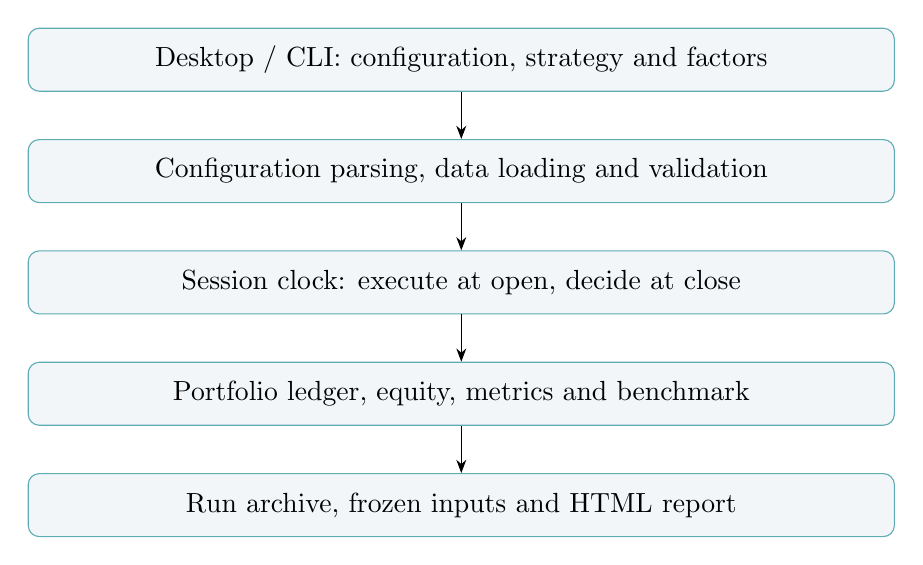
\begin{tikzpicture}[node distance=6mm,box/.style={draw=teal!65,fill=pale,rounded corners,minimum width=11cm,minimum height=8mm,align=center},>=Stealth]
\node[box] (a) {Desktop / CLI: configuration, strategy and factors};
\node[box,below=of a] (b) {Configuration parsing, data loading and validation};
\node[box,below=of b] (c) {Session clock: execute at open, decide at close};
\node[box,below=of c] (d) {Portfolio ledger, equity, metrics and benchmark};
\node[box,below=of d] (e) {Run archive, frozen inputs and HTML report};
\draw[->] (a)--(b);\draw[->] (b)--(c);\draw[->] (c)--(d);\draw[->] (d)--(e);
\end{tikzpicture}
\end{center}
The strategy specifies desired holdings. The engine determines execution time, price, quantities and costs. A factor only computes a feature from available history. This separation makes a change in the investment rule distinguishable from a change in the execution model.

\subsection{Top-level directories}
The table includes business directories and generated artifacts found in the current checkout. Finder may hide names beginning with a dot.
\begin{longtable}{p{0.29\linewidth}p{0.65\linewidth}}
\toprule Directory & Purpose and maintenance considerations\\\midrule\endhead
\path{src/quantlab/} & Installable Python core: data, engine, analytics, reports and application entry points.\\
\path{strategies/} & User strategies and an inert template. Preserve the rule specification and version when editing.\\
\path{factors/} & Approved pure feature calculations. Dependencies are explicitly bound, not automatically executed as a library of signals.\\
\path{configs/} & YAML experiment definitions; \path{examples/} contains the basic example. Separate configurations preserve old conditions.\\
\path{data/raw/} & Local original/frozen input, including synthetic sample data and historical market Parquet files. Keep their provenance distinct.\\
\path{data/processed/}, \path{data/cache/}, \path{data/metadata/} & Organizational locations for transformed data, caches and provenance. Actual use depends on the configuration and script; every run need not use every directory.\\
\path{runs/} & Independent experiment archives. These are evidence for analysis and reproduction, not disposable caches.\\
\path{desktop/} & React/TypeScript UI and Tauri shell. Its \path{src/} holds frontend code and \path{src-tauri/} holds Rust.\\
\path{scripts/} & Sample generation, data validation, clean-install checks and independent arithmetic auditing.\\
\path{tests/} & Offline automated tests, including small hand-checkable data in \path{fixtures/}.\\
\path{researchProject/} & Standalone studies with code, data, results and reports. Do not assume identical semantics to the core engine.\\
\path{validation/} & Earlier acceptance and research logs. Historical evidence is not a new verification of today's code.\\
\path{dist/}, \path{build/} & App/wheel deliverables and build intermediates. Source changes require rebuilding the affected deliverable.\\
\path{.quantlab-desktop/} & Desktop job snapshots and logs. Do not clean it during a run; cancellation may leave intermediate files.\\
\path{.venv/}, \path{.wheelhouse/} & Python environment and locally cached dependency wheels. A virtual environment is generally not portable by copying it.\\
\path{.git/} & Version history and remote configuration, not research data.\\
\path{.pytest_cache/}, \path{.ruff_cache/} & Rebuildable testing/tool caches, distinct from archived experiments.\\
\bottomrule
\end{longtable}

\subsection{Core modules and root files}
Within \path{src/quantlab/}, \path{data/} handles calendars, input checks and truncated views; \path{strategy/} defines contracts, context, loading and validation; \path{engine/} owns the clock, execution, orders and ledger; \path{costs/} implements commission and slippage; \path{metrics/} defines statistical conventions; \path{report/} builds charts and HTML; and \path{utils/} supports serialization, paths and logging.

\path{config.py} parses strict configurations, \path{cli.py} exposes commands, \path{archive.py} creates run archives, and \path{desktop_bridge.py} provides UI file, configuration, job and result operations. \path{types.py} contains shared types/exceptions; package initialization files provide Python package entry points.

At the root, \path{pyproject.toml} defines package metadata and dependency ranges; \path{requirements.lock} pins the accepted environment; \path{README.md} provides quick instructions; and \path{AGENTS.md} records development constraints and approved strategy rules. The V4 work document is the original specification. Acceptance documents and \path{DESKTOP_PROGRESS.md} are historical records. Resolve discrepancies by inspecting current code, tests and the specific archived experiment.

\chapterpage
\section{Installation and the first run}
\subsection{Prepare the Python environment}
The package declares Python 3.12 or newer. First inspect an existing environment rather than recreating it unnecessarily:
\begin{lstlisting}[language=bash]
cd /Users/yusa/ChatGPTWorkSpace/QuantLab
source .venv/bin/activate
python --version
python -m pip check
quantlab --help
\end{lstlisting}
For a new environment, select the intended Python interpreter and then run:
\begin{lstlisting}[language=bash]
python3.12 -m venv .venv
source .venv/bin/activate
python -m pip install -r requirements.lock
python -m pip install -e '.[dev]'
python -m pytest -q
\end{lstlisting}
Editable installation makes changes under \path{src/} effective in that environment. A dependency lock file is not a cross-platform installer: offline installation also needs compatible wheels. The current virtual environment may reference an external Python runtime. If that runtime is removed or moved, rebuild the environment rather than only changing its activation script.

\subsection{An offline smoke test}
\begin{lstlisting}[language=bash]
python scripts/make_sample_data.py
python scripts/validate_data.py configs/default.yaml
quantlab strategies validate \
  strategies/fixed_weight_buy_and_hold.py \
  --config configs/examples/fixed_weight_buy_and_hold.yaml
quantlab backtest run \
  --config configs/examples/fixed_weight_buy_and_hold.yaml
\end{lstlisting}
The generator creates synthetic prices with a fixed seed. Symbols such as AAPL, TSLA and SPY do not make those generated prices real historical observations. Use this example to verify installation and the complete pipeline, not to draw investment conclusions.

The command prints the run directory and final equity. Replace \code{RUN_ID} below with the actual identifier:
\begin{lstlisting}[language=bash]
quantlab report open RUN_ID
\end{lstlisting}
When working outside the project root, use \code{--runs-dir /absolute/path/to/runs}. Alternatively, open the archive's \path{report.html} directly in a browser.

\subsection{Use the existing historical dataset}
Real market data are not distributed with this release. In a fresh clone, first generate the synthetic sample and select its basic configuration in the App. The historical experiments below require locally prepared data at the configured paths.

The existing weekly research configurations point to a local Yahoo historical Parquet file. Running them does not download fresh data. Validate and run as follows:
\begin{lstlisting}[language=bash]
python scripts/validate_data.py \
  configs/weekly_equal_weight_aapl_tsla_2020_2025.yaml
quantlab strategies validate \
  strategies/weekly_equal_weight_aapl_tsla.py \
  --config configs/weekly_equal_weight_aapl_tsla_2020_2025.yaml
quantlab backtest run \
  --config configs/weekly_equal_weight_aapl_tsla_2020_2025.yaml
\end{lstlisting}
This configuration begins with a cash baseline on 3 January 2020 so the first instruction can execute at the open on 6 January. Moving the configured start directly to the intended purchase day changes available history, the first execution and the performance baseline.

\section{Desktop application workflow}
\subsection{Open and connect}
Open \path{dist/QuantLab.app} in Finder. If the workspace is not detected, enter the project root's absolute path in Workspace Settings. It should contain \path{pyproject.toml}, \path{src/quantlab/}, strategies, configurations and a working \path{.venv/bin/python}. The packaged App does not require the browser development server.

The sidebar provides the research workbench, run history, data catalog and workspace settings. Dark/light theme selection changes appearance only. The data catalog primarily lists local files; it is not a full data procurement, online refresh or cleaning platform.

\subsection{Select, edit, configure and run}
\begin{enumerate}
\item Select a configuration preset close to the intended experiment. Inspect the strategy, universe, benchmark and dates.
\item Select a Python strategy from \path{strategies/}. Read its actual rule and recheck parameter compatibility after switching files.
\item Select a factor to open it in the editor. If the strategy imports it, also bind the dependency and call its function in code. Opening a factor alone does not create trades.
\item Edit the source and save with the button or Command+S. Multiple documents can remain as tabs. A new strategy starts from the existing template; a new factor is an unimplemented stub.
\item Set dates, capital, universe, benchmark and local data. Expand advanced settings for JSON parameters, sizing and trading costs.
\item Validate the strategy, then run. The application saves edits, validates the configuration and freezes the source used for that job. Inspect logs or cancel when needed.
\item Confirm the result's run identifier, then inspect equity, metrics, fills and the full report.
\end{enumerate}

\subsection{Distinguish source, form values and results}
Saving code updates local Python files. Editing the form does not automatically overwrite the original YAML configuration; the experiment values are preserved in the run snapshot. Create or edit a YAML file under \path{configs/} to keep a reusable preset.

An old curve does not mean the current edits have been tested. Only a new successful run corresponds to the new inputs. The history view returns at most the latest 100 entries, and the fill table displays at most 2,000 rows. Older archives and complete fills remain on disk. Damaged entries are isolated as failures, failure markers take precedence, and successful records require complete metadata.

Content fingerprints prevent silently overwriting a file changed by another editor. Copy any draft you need to keep, reload the disk version and merge intentionally. Cancellation does not make partial output a valid result; a leftover directory alone is not evidence of a successful run.

\subsection{Development and packaging}
Using an existing App does not require Node or Rust. Development/rebuilding requires a Node.js version supported by Vite 6, npm, Rust/Cargo and macOS developer tools. This release updates Vite to the compatible 6.4.5 patched line and source-map-js to 1.2.2; the release-time npm audit reported zero known vulnerabilities:

\begin{lstlisting}[language=bash]
cd desktop
npm ci
npm run desktop
# Build the production macOS app:
npm run bundle
\end{lstlisting}
For a browser-only development preview:
\begin{lstlisting}[language=bash]
QUANTLAB_WORKSPACE=/Users/yusa/ChatGPTWorkSpace/QuantLab npm run dev
\end{lstlisting}
The preview binds to \code{127.0.0.1:1420}. The native application calls Python through Tauri IPC. The new bundle is produced at \path{desktop/src-tauri/target/release/bundle/macos/QuantLab.app}. Test it, quit the old App and then replace the delivered copy. Editing source does not update an already packaged binary.

\chapterpage
\section{Turn an idea into an executable experiment}
\subsection{Specify the rule before implementation}
A verbal request should define the tradable symbols and observable benchmark; exact arithmetic and thresholds; initial allocation; signal interval; decision and execution times; holiday handling; cash and position sizing; costs; start/end dates; missing-data behavior; parameters; and any prohibition on automatic optimization.

For example, ``equal weight every Monday'' is ambiguous between Monday-open execution and Monday-close decisions for Tuesday execution. The approved AAPL/TSLA strategy decides at the final close of the preceding trading week and executes at the first open of the next week.

A typical implementation delivers \path{strategies/name.py} and \path{configs/name.yaml}, plus \path{factors/name.py} only when a new feature is needed. An engine change must be identified and tested separately. Neither a developer nor an AI assistant should silently change the rule to improve returns. The workflow is specification, implementation, validation, backtest, audit and reporting.

\subsection{The strategy interface}
Copy \path{strategies/_template.py}, or create a new strategy in the App. This minimal inert skeleton is an interface example, not an additional investment rule:
\begin{lstlisting}[language=Python]
from quantlab.strategy.base import BaseStrategy

STRATEGY_META = {
    "name": "my_strategy", "version": "0.1.0",
    "description": "Document the exact approved rule",
}

class Strategy(BaseStrategy):
    def warmup_bars(self):
        return 0

    def generate_target_weights(self, dt, data, ctx):
        return None

    def decision_metadata(self):
        return {}

def build_strategy(params):
    return Strategy(params)
\end{lstlisting}
\code{build_strategy(params)} creates the instance. The base class copies parameters, and the strategy may keep its own historical state. \code{decision_metadata()} supplies auditable explanations such as factor values and trigger reasons; it must not submit extra orders.

Return values have distinct meanings: \code{None} means no new instruction; an empty dictionary means an all-cash target; a nonempty dictionary specifies the whole target portfolio, so omitted existing holdings have a zero target. Weights must be finite, nonnegative, within the tradable universe and inside position/gross-exposure limits. A sum below one leaves a cash target. Subsequent market drift does not trigger automatic enforcement of the target weights.

\subsection{Available observations}
\begin{longtable}{p{0.43\linewidth}p{0.51\linewidth}}
\toprule Interface & Meaning\\\midrule\endhead
\code{data.history(symbol, bars=None, end=None)} & A copy of history visible at the decision cutoff, optionally limited by count and end date.\\
\code{data.current(symbol)} & The current visible bar or \code{None}; missing data must be handled.\\
\code{data.as_of} & The view's session cutoff.\\
\code{ctx.cash}, \code{ctx.equity} & Read-only current cash and equity.\\
\code{ctx.positions}, \code{ctx.universe} & Read-only quantity mapping and permitted tradable symbols.\\
\code{ctx.next_session_date} & The next session from known calendar metadata, not a future market observation.\\
\code{ctx.seed}, \code{ctx.execution_sizing} & Random seed and active execution-sizing mode.\\
\bottomrule
\end{longtable}
Benchmark history is observable without making the benchmark tradable. Warmup counts only observable bars inside the chosen backtest interval. The engine does not automatically load training history before that interval; configure enough history for the rule.

Strategies must not download data, access future information, import private engine objects or mutate the ledger. Validation checks common prohibited imports and file I/O, but it proves neither arbitrary Python safety nor investment efficacy.

\subsection{Bind configuration and run}
Copy an existing YAML file and edit \code{strategy.path}, \code{params}, the universe and data path. YAML-relative paths resolve from the YAML file's directory. An explicit CLI \code{--strategy} path resolves from the current shell directory and overrides the YAML strategy.
\begin{lstlisting}[language=bash]
quantlab strategies validate strategies/my_strategy.py \
  --config configs/my_strategy.yaml
quantlab backtest run --config configs/my_strategy.yaml
\end{lstlisting}
Passing validation establishes a basic contract only. Inspect edge cases, key decision dates, holdings and cash, and check that the observed output matches the written rule.

\section{Factors and the existing strategies}
\subsection{A factor is not a trading policy}
A factor is a calculated feature. A strategy uses features, timing and portfolio state to decide trades. For example, the daily AAPL-minus-SPY return spread is
\[
 f_t=\left(\frac{P^{A}_{t}}{P^{A}_{t-1}}-1\right)
     -\left(\frac{P^{M}_{t}}{P^{M}_{t-1}}-1\right).
\]
Prices here use the system's adjusted series. This is neither a beta-adjusted residual nor direct evidence of overvaluation/undervaluation. A threshold of \(\pm0.01\) means a difference of one percentage point, not an additional percentage scaling of the spread.

The factor determines neither trade size nor execution time. Different strategies can use the same feature. Conversely, restoring fixed 50/50 weights weekly needs no predictive factor, so it does not inherently create a factor-library file.

\subsection{The current return-spread factor}
\path{factors/return_spread.py} provides \code{daily_return_spread} and \code{weekly_return_spread}. The daily function uses two synchronized daily closes. The weekly function compares the final closes of two adjacent completed trading weeks. A weekly return is neither the last daily return nor simply the arithmetic sum of daily returns.

Call the weekly function only after the strategy has established that the current close is the last session of the week; otherwise a partial week could be treated as complete. Insufficient history returns \code{None}; unsynchronized endpoints and nonpositive prices fail explicitly. The result includes endpoint dates, asset/benchmark returns and their spread for auditing.

Example binding in a YAML file under \path{configs/}:
\begin{lstlisting}
strategy:
  path: ../strategies/aapl_weekly_relative_reversal.py
  params:
    start_date: '2020-01-06'
    end_date: '2025-12-31'
    threshold: 0.01
  rebalance_schedule: daily
  factor_paths:
    factors.return_spread: ../factors/return_spread.py
execution:
  sizing: decision_relative
\end{lstlisting}
This is a fragment, not a replacement for the other sections of the full configuration. The strategy imports \code{weekly_return_spread} from \code{factors.return_spread}. The loader explicitly binds, checks and freezes the module's source. It does not execute every file found in the factor directory.

\subsection{Distinguish the existing rules}
\begin{longtable}{p{0.43\linewidth}p{0.51\linewidth}}
\toprule File / experiment & Implemented behavior\\\midrule\endhead
\path{fixed_weight_buy_and_hold.py} & Submit the initial configured allocation, then do not actively rebalance. The basic example is 50/50 AAPL/TSLA; the half-AAPL control reuses this implementation.\\
\path{weekly_equal_weight_aapl_tsla.py} & Begin on 6 January 2020 and restore 50/50 targets at each week's first session open; no factor needed.\\
\path{aapl_weekly_relative_reversal.py} & Start with half the cash invested in AAPL. Later weekly spread below -1pp buys with half remaining cash; above +1pp sells half the shares; otherwise hold.\\
\path{_template.py} & Inert starting point returning \code{None}, not a validated investment rule.\\
\bottomrule
\end{longtable}
The reversal strategy gives initial entry precedence, without a simultaneous factor trade. Cash earns no interest; purchase budgets include commissions; sales round down. Equality at the threshold, with a \(10^{-12}\) boundary tolerance in code, produces no trade. The rule requires \code{decision_relative}; ordinary target-weight execution is not interchangeable with it.

\chapterpage
\section{Data, configuration and execution semantics}
\subsection{Data contract and adjustment}
Local input is long format, one symbol/session per row:
\begin{lstlisting}
date,symbol,open,high,low,close,volume,adj_close
\end{lstlisting}
The date is a timezone-naive session label; decision and fill timestamps use UTC. Data must cover the tradable universe and benchmark under the XNYS calendar. Duplicate symbol/date pairs, invalid prices, negative volume, non-session dates and absent required symbols fail explicitly.

In \code{adjusted} mode, all OHLC values are scaled by \(a_t=\text{adj\_close}_t/\text{close}_t\). Dividends and splits are not credited again, and volume retains its source value. Integer quantities are adjusted research units, not literal historical raw shares. \code{raw} mode does not process corporate actions and rejects explicitly nonzero dividends or nontrivial split indicators. Missing action disclosures can still bias a raw-price study.

When refreshing data, preserve the old file and create a new version with source, download date, interval, adjustment policy and validation results. Vendors can revise adjusted history; frozen inputs are necessary to explain result changes. The optional Yahoo adapter is a convenience source, not a unique authority. Install \code{'.[online]'} and explicitly choose \code{data.provider: yahoo} when required. The desktop workflow primarily uses local files.

\subsection{Configuration map}
\begin{longtable}{p{0.31\linewidth}p{0.63\linewidth}}
\toprule Section & Controls\\\midrule\endhead
\code{backtest} & Start/end dates, positive initial capital and USD base currency.\\
\code{data} & Provider, path, daily frequency, adjustment mode, benchmark, provenance and extreme-return warning threshold.\\
\code{universe} & A nonempty unique symbol list and fixed-list/current-constituent provenance.\\
\code{strategy} & Source, parameters, decision-eligibility schedule and factor module-to-source bindings.\\
\code{execution} & Close decisions, next-open execution, integer quantities and sizing mode.\\
\code{commission}, \code{slippage} & Fee model, minimum fee and basis-point slippage. One basis point is 0.01\%.\\
\code{portfolio} & No shorting or negative cash; single-position and gross-exposure limits.\\
\code{analytics} & Annualization sessions (default 252), risk-free rate and rolling window.\\
\code{report} & Report generation, automatic opening and output root.\\
\code{reproducibility} & Random seed; a seed alone does not replace data/code snapshots.\\
\bottomrule
\end{longtable}
Strict Pydantic models reject unknown fields and nonfinite values. Duplicate YAML keys also fail. Relative paths are based on the YAML location, not a UI navigation location.

\subsection{Daily event order and weekly timing}
\begin{enumerate}
\item At the open, process the target produced at the preceding session's close.
\item Mark existing holdings at current opens and freeze equity for target conversion.
\item Apply slippage and integer sizing; sell first, then buy in alphabetical symbol order.
\item Deterministically reduce unaffordable buys and cancel the remainder. No borrowing is allowed, and zero fills incur no minimum commission.
\item At the close, value the portfolio, create a truncated history view, invoke the strategy and record the end-of-day state.
\end{enumerate}
\code{rebalance_schedule: weekly} means decision eligibility at the first session's close each week, not Monday-open execution. The existing Monday-open strategies use \code{daily} to check whether the next session enters a new week and emit targets only at that boundary. Known calendar metadata is available in advance; future prices are not.

\subsection{Two execution-sizing modes}
\code{target_weights} converts desired weights into integer quantities using opening equity. A 50/50 target need not produce exact equal values because of costs, slippage, rounding and cash constraints.

\code{decision_relative} freezes a cash/share fraction implied by the change in close-time weights, then executes that fraction at the next open. This preserves ``spend half the remaining cash'' across an overnight gap. It currently supports one tradable symbol, as required by the AAPL reversal, rather than being a general multi-asset sizing algorithm.

\subsection{Costs and missing data}
Commissions support zero, per-share with a minimum, and notional basis points. Slippage supports zero or basis points, increasing purchase prices and reducing sale prices. It is already embedded in fill prices and must not be charged to cash again. Purchase commissions enter average cost; net sale proceeds determine realized P\&L.

Missing execution bars, invalid opens or zero volume cancel orders without future-price substitution. A missing held-position bar uses the last known mark with a warning; a missing benchmark bar fails the run. Targets still pending on the final day are cancelled, but terminal holdings are not forcibly liquidated.

Final daily volume serves only as a zero-volume tradability flag. It is not known at the real open, so this is an explicit daily-model assumption, not an intraday liquidity simulation. The ledger checks
\[
E_t=C_t+MV_t=E_0+\mathrm{RealizedPnL}_t+\mathrm{UnrealizedPnL}_t.
\]

\section{Interpret performance correctly}
Before examining returns, verify provenance, dates, first purchase, benchmark, costs and warnings. A smaller drawdown can result from lower equity exposure rather than better timing. Compare the reversal with the matching initial-half-AAPL buy-and-hold control as well as observing SPY.

Let \(E_t\) be closing equity and \(r_t=E_t/E_{t-1}-1\). The first session close is a cash baseline; return statistics omit its placeholder zero. Principal definitions are
\begin{align*}
R_{\rm total}&=E_T/E_0-1,\\
\mathrm{CAGR}&=(E_T/E_0)^{1/Y}-1,\quad Y=\frac{d_T-d_0}{365.25},\\
\sigma_{\rm ann}&=s(r_t)\sqrt{252},\\
\mathrm{Sharpe}&=\frac{\overline{r_t-r_f}}{s(r_t-r_f)}\sqrt{252},\\
\mathrm{MDD}&=\min_t\left(\frac{E_t}{\max_{u\le t}E_u}-1\right).
\end{align*}
The annualization count is configurable; \(s\) is the sample standard deviation and the annual risk-free rate is converted geometrically to a daily rate. Sortino uses the square root of the mean squared negative excess return over all observations. Calmar divides CAGR by absolute maximum drawdown. Drawdown duration uses calendar days, ending an unrecovered episode at the final observation.

Turnover uses two-sided filled notional divided by previous-close equity, then annualizes by the number of return intervals; there is no division by two. Average exposure and cash include the initial cash-only session. Beta, alpha, tracking error and information ratio use aligned benchmark daily returns. The benchmark is a costless, fractional-share buy-and-hold curve from the first session close, not an executable copy of the strategy's account.

Undefined ratios are \code{null}/N/A, not zero. Fill count is not completed round-trip count, and the system does not invent a round-trip win rate for buy and hold. HTML reports embed their images for offline reading. Use CSV/Parquet/JSON records, not chart pixels, for numerical audits.

\chapterpage
\section{Archives, reproduction and independent audit}
\subsection{What a run preserves}
Run directory names include UTC time, strategy name and a digest; new runs do not overwrite earlier experiments. The following files establish what actually ran:
\begin{longtable}{p{0.43\linewidth}p{0.51\linewidth}}
\toprule Artifact & Role\\\midrule\endhead
\path{config.snapshot.yaml} & Resolved configuration redirected to frozen inputs.\\
\path{config.original.json} & Initially resolved configuration, including original paths.\\
\path{strategy.snapshot.py}, \path{factors.snapshot/} & Strategy and explicitly bound factor sources.\\
\path{data.snapshot.parquet} & Actual pre-adjustment input panel, avoiding fresh downloads.\\
\path{code.snapshot/}, \path{requirements.snapshot.txt} & Engine source, installation description and dependency versions.\\
\path{metadata.json}, \path{manifest.json} & Environment, Git state, fingerprints and file SHA-256 values. The manifest excludes itself and the still-written log.\\
\path{equity.csv}, \path{returns.csv}, \path{benchmark.csv} & Equity, returns and benchmark records.\\
\path{decisions.csv}, \path{orders.csv}, \path{fills.csv} & Decision explanations, requested/cancelled/executed orders and costs.\\
\path{positions.parquet} & Daily holdings.\\
\path{summary.json}, \path{metrics.json}, \path{warnings.json} & Summary, complete metrics and warnings.\\
\path{report.html}, \path{logs.txt}, \path{reproduce.sh} & Human-readable report, logs and reproduction entry point.\\
\path{failure.json} & Failure marker; the directory is not a successful experiment.\\
\bottomrule
\end{longtable}
HTML can be absent when report generation is disabled. A Git commit alone is insufficient when source has uncommitted edits; frozen source and hashes are more direct evidence. Back up the complete archive rather than only screenshots or a PDF.

\subsection{Rerun and migrate}
Within the same environment:
\begin{lstlisting}[language=bash]
sh runs/RUN_ID/reproduce.sh
\end{lstlisting}
This creates a new run. For a different environment, create a fresh virtual environment, install that archive's \path{requirements.snapshot.txt} and \path{code.snapshot/}, then use its reproduction command. Moving archives can invalidate absolute paths. Preserve originals, save a separate configuration with corrected paths and document the changes. Do not substitute today's engine for historical source without disclosure.

Identical inputs, rules and environments should preserve economic results; cross-platform floating-point behavior need not produce byte-identical files. Compare dates, quantities, fees, daily equity and metrics, not just terminal return.

\subsection{The existing independent audit}
\begin{lstlisting}[language=bash]
python scripts/audit_weekly_relative_reversal.py runs/RUN_ID
\end{lstlisting}
This script independently recomputes signals, cash/share arithmetic and daily equity for the existing weekly reversal without importing its strategy or engine implementation. It assumes that rule and its cost conventions. It is not a universal audit tool; a changed rule requires a correspondingly independent calculation.

\section{Using the standalone research studies}
Start with \path{researchProject/RESEARCH_INDEX.md}. The current studies ask:
\begin{enumerate}
\item \path{01_aapl_tsla_rebalancing/}: how target weights and calendar rebalancing frequency change AAPL/TSLA results.
\item \path{02_threshold_partial_rebalancing/}: how threshold triggers and partial corrections affect trading, tracking and performance.
\item \path{03_time_and_asset_robustness/}: whether results persist across entry dates, holding horizons and asset pairs.
\item \path{04_rebalancing_mechanisms/}: how diversification growth differs from net outperformance of buy and hold.
\end{enumerate}
Follow each study's README and audit instructions. Read its report, protocol, data dictionary, results and code rather than trying to choose its report file in the App. Later studies contain separate calculation engines; similar names do not establish identical implementation details.

Study 04 explicitly separates frictionless close-to-close identities, synthetic experiments and the original opening-execution convention. Mathematical decomposition terms are not substitutes for net opening-execution performance. Fixed asset selection, overlapping windows and parameter comparisons do not automatically establish out-of-sample evidence. Promoting a research idea to a supported strategy requires a precise rule, strategy/factor contracts, tests and verification against the main engine.

\chapterpage
\section{Maintenance, verification and delivery}
\subsection{A disciplined change process}
\begin{enumerate}
\item Record the purpose and expected behavior; identify whether the change concerns data, strategy, engine or UI.
\item Preserve the old configuration and a reference run; version source and do not overwrite historical data files.
\item Implement the smallest necessary change. Material engine changes require tests that detect meaningful failures, including preserved no-look-ahead checks.
\item Run focused tests and the full suite; perform a representative offline end-to-end run when appropriate.
\item For trading-semantic changes, compare orders, fills, equity and costs and explain why results changed.
\item Update documentation/configuration notes; rebuild and verify the native App after interface changes.
\end{enumerate}

\subsection{Routine verification commands}
\begin{lstlisting}[language=bash]
python -m pytest -q
python -m pip check
# Desktop checks, from desktop/:
npm ci
npm run build
cargo check --manifest-path src-tauri/Cargo.toml
npm run bundle
\end{lstlisting}
The full Python suite was rerun for this manual on 22 October 2026: \textbf{136 tests passed}. This is a dated check, not a guarantee about future edits or a substitute for native release QA. Coverage includes accounting, costs, missing data, contracts, no-look-ahead behavior, configuration, archive reproduction and desktop bridging.

\path{scripts/check_clean_install.py} verifies wheel installation, tests and an offline example in a temporary environment. It requires a built project wheel under \path{dist/} and all necessary platform dependencies under \path{.wheelhouse/}. Missing preparation is not evidence of a strategy failure.

\subsection{Dependencies, backups and publication}
Upgrade dependencies in a fresh environment, respect \path{pyproject.toml} ranges, update appropriate lock files and run regression checks. The frontend uses \path{package-lock.json}; Rust uses \path{Cargo.lock}. Check native interface compatibility rather than upgrading one side in isolation.

Back up source, configurations, original data, complete important run archives and research protocols. Environments/build caches are reconstructible, but a fully offline recovery also needs compatible wheels and installation tools. Ensure no job is running before cleanup. \path{runs/} and \path{.quantlab-desktop/} have different roles.

On 22 October 2026, the owner authorized publishing the current simple strategies and factor. Release 2026.10.22 includes the application, desktop source, configurations, tests and manuals. Independent \path{researchProject/} studies, real market data, run archives, environments and caches are excluded. The existing GitHub repository was public when checked for this release; its visibility is retained. Inspect the export list and history: \path{.gitignore} does not remove previously committed material. See \path{PROJECT_SCOPE.md} for the release boundary.

\subsection{Maintaining this manual}
Each edition is a self-contained LaTeX source with no external image dependencies. The Chinese edition uses XeLaTeX with system Chinese fonts or Fandol fallbacks; the English edition uses TeX Gyre fonts. Compile twice after changes to resolve the contents and references. Check for overflow, missing glyphs and broken code. Put auxiliary output in a temporary directory; retain only the source and PDF in the final cn/en directories.

\section{Troubleshooting and operating checklist}
\begin{longtable}{p{0.27\linewidth}p{0.67\linewidth}}
\toprule Symptom & First checks\\\midrule\endhead
Command missing / import fails & Working directory, activated environment, Python version, editable install and \code{quantlab --help}.\\
App cannot connect & Correct project root, working \path{.venv/bin/python}, moved paths and complete dependencies.\\
Invalid configuration & Unknown/duplicate YAML keys, date order, parameter types and YAML-relative paths.\\
Strategy validation fails & Metadata, base class, factory, returned weights, prohibited imports, factor bindings and sizing mode.\\
Factor module missing & The \code{factor_paths} module name must match the import and bind the intended source.\\
No fills & No target, insufficient warmup, inactive dates, inadequate cash, or cancelled missing-open/zero-volume orders. Inspect decisions and orders.\\
Weekly execution a day late & Confusion between weekly close-time eligibility and Monday-open execution; inspect the next-session date.\\
Weights not exactly equal & Integer quantities, costs, opening gaps and cash constraints; distinguish targets from realized holdings.\\
Unchanged curve & A historical run may still be displayed; confirm a new successful identifier after edits.\\
Save conflict & External source changed; preserve the draft, reload and merge rather than force-overwrite.\\
Run fails / report absent & Inspect failure marker, logs and report switch. Directory existence alone does not prove success.\\
Reproduction differs & Compare data, source, parameters, versions and seed; check relocated paths and use of a newer engine.\\
Source updated, App unchanged & Rebuild the bundle and open the new copy rather than the previous binary.\\
\bottomrule
\end{longtable}
Before presenting research, confirm that the rule was fixed in advance, data provenance is clear, information timing is valid, costs are explicit, exceptions are disclosed, controls are appropriate and complete archives are preserved. Report poor performance honestly instead of automatically adjusting thresholds until a favorable backtest appears.

\appendix
\section{Source basis and version interpretation}
This manual was checked on 22 October 2026 against the local \path{README.md}, \path{AGENTS.md}, \path{pyproject.toml}, configurations, core configuration/CLI modules, strategy base/context, factor functions, performance implementation, desktop bridge, \path{desktop/README.md}, research index and utility scripts. The application version is \code{2026.10.22}, identified by Git tag \code{v2026.10.22}. Resolve that tag for the exact release commit. Review scope and evidence are recorded in \path{AUDIT_2026.10.22.md}.

Implementation takes precedence over stale wording. The older README's V2 roadmap and ``single official example'' wording describe an earlier stage; approved additional strategies, the desktop app and research studies now exist. This manual does not infer unimplemented live trading, generic automatic optimization, a complete factor-evaluation platform or a self-contained cross-machine installer from those additions.
\end{document}
